\documentclass[12pt]{article}
%\usepackage{epsf,epic,eepic,eepicemu}
%\documentstyle[epsf,epic,eepic,eepicemu]{article}
%\usepackage[cp1250]{inputenc}
\usepackage[utf8]{inputenc}
\usepackage[czech, english]{babel}
\usepackage{czech}
\usepackage[T1]{fontenc} 
\usepackage{verbatim}
\usepackage{graphicx}
\usepackage{hyperref}
\usepackage{lmodern}
\usepackage{float}

\makeindex

\begin{document}
%\oddsidemargin=-5mm \evensidemargin=-5mm \marginparwidth=.08in
%\marginparsep=.01in \marginparpush=5pt \topmargin=-15mm
%\headheight=12pt \headsep=25pt \footheight=12pt \footskip=30pt
%\textheight=25cm \textwidth=17cm \columnsep=2mm \columnseprule=1pt
%\parindent=15pt\parskip=2pt

\begin{center}
\bf Semestrální projekt MI-PAP 2010/2011:\\[5mm]
    Paralelní řadící algoritmy\\[5mm]
    Pavel Benáček\\   
    Tomáš Čejka\\[2mm]
magisterské studijum, FIT ČVUT, Kolejní 550/2, 160 00 Praha 6\\[2mm]
\today
\end{center}
\newpage

\tableofcontents
\listoftables
\newpage
\section{Definice problému a popis sekvenčního algoritmu}
\subsection{Zadání}
Podle zadání semestrální práce je úkolem implementace aspoň tří z následujících
řadících algoritmů: Shearsort, 3D sort, Sudo-lichý Mergesort a Bitonic sort.

Pro řešení jsme si vybrali algoritmy Shearsort, Sudo-lichý Mergesort a Bitonic sort.

Pro účely měření času běhu výsledných programů a porovnání paralelních algoritmů se sekvenčním
řazením jsme si implementovali sekvenční algoritmus Mergesort a ten vzali jako referenční sekvenční
řešení.

Semestrální práce spočívala v implementaci vybraných řadících algoritmů jako sekvenční řešení, paralelní
řešení na počítači se sdílenou pamětí s použítím knihovny OpenMP a následně s využitím technologie CUDA
společnosti NVIDIA\textsuperscript{\tiny{\textregistered}}.

\subsection{Řešení}
Vytvořili jsme si základní moduly \textbf{Loader} a \textbf{Array} (případně ještě pro Shearsort 
\textbf{Array2D}), které sdílíme mezi jednotlivými implementacemi algoritmů.

Modul Array se stará o uchování načtených dat a při načtení se stará o zvětšování alokované paměti 
v případě potřeby. Modifikace Array2D umožňuje mapování jednorozměrného pole na dvourozměrné.

Loader čte předané parametry programu a nastavuje na jejich základě počet prvků k seřazení a počet
spouštěných vláken. Loader dokáže vygenerovat pseudonáhodnou posloupnost prvků nebo načíst data ze zadaného
souboru.

Přikompilování těchto modulů nám vytváří stejné rozhraní u všech programů.

Implementací paralelních algoritmů Bitonicsort a Even-Odd mergesort vznikly i prototypy sekvenční.
Tyto programy jsme rovněž zařadili do měření.

Měření jsme prováděli plně automatizovaně - v adresáři /utils jsme pro ten účel vytvořili skripty,
které nám vytvoří strukturu adresářů /tests, do které podle počtu vlánek a objemu dat vygeneruje
skripty pro zadání úlohy do fronty.

Nad touto strukturou adresářů je možné jednoduše provádět zařazení úloh do fronty i vybrání naměřených
výsledků.

\section{Popis paralelního algoritmu a jeho implementace v OpenMP}
\subsection{Sudo-lichý mergesort}
Algoritmus Sudo-lichý mergesort je navržen na strukturu řadící sítě, kterou si můžeme představit jako
systém s distribuovanou pamětí, který obsahuje množinu procesorů uspořádaných do mřížky a vhodně pospojovaných.

Algoritmus funguje tak, že na vstup systému se přivede množina dat, která se během průchodu sítí seřadí.

Řešení paralelizace s knihovou OpenMP pracuje na počítači se sdílenou pamětí, není potřeba množinu dat
rozdělovat na dílčí části a distribuovat/rozkopírovat je mezi procesory. Místo toho jsou veškerá data
umístěna v paměti v jednom poli a jednotlivá paralelní vlákna přistupují k disjunktním oblastem sdíleného
pole.

Snažili jsme se o co nejrovnoměrnější rozdělení dat mezi vlákna, takže data virtuálně rozdělíme na začátku
programu na stejné části, jejichž počet je rovný nějaké mocnině dvou a jednotlivá vlákna seřadí tuto podposloupnost
dat. Tento přístup je možný díky rekurzivní povaze algoritmu a řadících sítí.
Po seřazení podposloupností je potřeba ještě provést jejich sloučení. Sloučení se provádí v logaritmickém čase,
protože díky půlení posloupnosti se slučuje vždy \(log n\) podposloupností.

\subsection{Bitonic sort}
Bitonic sort vytváří v posloupnosti dat dvě podposloupnosti, kde jedna je nerostoucí a druhá neklesající.
V druhé fázi se dílčí podposloupnosti slévají až jsou nakonec data seřazená.

Rozdělování podposloupností probíhá na disjuktních částech posloupnosti, což umožňuje paralelizaci.
Ve smyčce, kterou procházíme pole dat se zvětšuje proměnná, určující rozestup mezi prvky.

\subsection{Shearsort}
Posledním implementovaným řadícím algoritmem je Shearsort. Algoritmus jsme realizovali 
s použitím sekvenčního algoritmu mergesort, který voláme na seřazení jednotlivých řádků a sloupců
mřízky, do které jsou data virtuálně rozdělena. Virtuálně proto, že používáme pro uložení dat jednorozměrné
pole a mapovací funkci, která umožňuje adresovat prvek matice souřadnicemi \emph{x} a \emph{y}.

Jednotlivé fáze algoritmu (sloupcové a řádkové) je nutné provést sekvenčně za sebou,
ale řazení řádků i sloupců v jedné fázy je možné spouštět najednou paralelně.

\section{Naměřené výsledky a vyhodnocení}
\subsection{Způsob měření}
Měření probíhalo za pomoci knihovní funkce \textbf{omp\_get\_wtime()}, která vrací čas běhu programu.
Uložením času na začátku výpočtu a jeho odečtením od času na konci výpočtu dostaneme dobu, kterou
algoritmus potřebuje na seřazení vstupních dat.

Vlastní zařazení našich programů do fronty na serveru \textbf{star} je popsané v sekci 1.2.

\subsection{Naměřené časy}

\subsubsection{Sekvenční Mergesort}
\begin{table}[H]
\begin{center}
\begin{tabular}{|r|r|r|r|}
\hline Množství dat (2\textsuperscript{n}) & Počet vláken & Čas \\ \hline
10 & 1 &  0,000236067 \\ \hline
10 & 1 &  0,000236629 \\ \hline
10 & 1 &  0,000001956 \\ \hline
16 & 1 &  0,022770800 \\ \hline
16 & 1 &  0,022806500 \\ \hline
20 & 1 &  0,449648000 \\ \hline
20 & 1 &  0,450177000 \\ \hline
24 & 1 &  8,545500000 \\ \hline
24 & 1 &  8,547720000 \\ \hline
26 & 1 &  37,555900000 \\ \hline
26 & 1 &  37,559000000 \\ \hline
\end{tabular} 
\end{center}
\caption{Mergesort}
\end{table}

\subsubsection{Sekvenční Even-Odd Mergesort}
\begin{table}[H]
\begin{center}
\begin{tabular}{|r|r|r|r|}
\hline Množství dat (2\textsuperscript{n}) & Počet vláken & Čas \\ \hline
10  & 1 & 0,000634586  \\ \hline
10  & 1 & 0,000634735  \\ \hline
10  & 1 & 0,000635005  \\ \hline
10  & 1 & 0,000001676  \\ \hline
16  & 1 & 0,098675900  \\ \hline
16  & 1 & 0,099481000  \\ \hline
16  & 1 & 0,100037000  \\ \hline
20  & 1 & 3,569340000  \\ \hline
24  & 1 & 118,748000000  \\ \hline
24  & 1 & 120,404000000  \\ \hline
24  & 1 & 130,860000000  \\ \hline
26  & 1 & 709,920000000  \\ \hline
26  & 1 & 735,275000000  \\ \hline
\end{tabular} 
\end{center}
\caption{Even-Odd Mergesort}
\end{table}


\subsubsection{Sekvenční Bitonic sort}
\begin{table}[H]
\begin{center}
\begin{tabular}{|r|r|r|r|}
\hline Množství dat (2\textsuperscript{n}) & Počet vláken & Čas \\ \hline
10  & 1 & 0,000650510 \\ \hline
16  & 1 & 0,091356500 \\ \hline
20  & 1 & 2,216730000 \\ \hline
24  & 1 & 50,019500000 \\ \hline
26  & 1 & 233,403000000 \\ \hline
\end{tabular} 
\end{center}
\caption{Bitonic sort}
\end{table}


\subsubsection{Bitonic sort}
\begin{table}[H]
\begin{center}
\begin{tabular}{|r|r|r|r|}
\hline Množství dat (2\textsuperscript{n}) & Počet vláken & Čas \\ \hline
10 & 2  & 0,000049379 \\ \hline
10 & 4  & 0,000057481 \\ \hline
10 & 8  & 0,000048540 \\ \hline
10 & 16 & 0,000058248 \\ \hline
10 & 32 & 0,000048400 \\ \hline
16 & 2  & 0,009313320 \\ \hline
16 & 4  & 0,015767700 \\ \hline
16 & 8  & 0,539144000 \\ \hline
16 & 16 & 0,006299840 \\ \hline
16 & 32 & 0,007108750 \\ \hline
20 & 2  & 0,199643000 \\ \hline
20 & 4  & 0,122328000 \\ \hline
20 & 8  & 0,288970000 \\ \hline
20 & 16 & 0,100444000 \\ \hline
20 & 32 & 0,096497300 \\ \hline
24 & 2  & 4,928480000 \\ \hline
24 & 4  & 3,395880000 \\ \hline
24 & 8  & 2,753720000 \\ \hline
24 & 16 & 2,713770000 \\ \hline
24 & 32 & 2,861780000 \\ \hline
26 & 2  & 24,432600000 \\ \hline
26 & 4  & 16,383700000 \\ \hline
26 & 8  & 13,385400000 \\ \hline
26 & 16 & 13,238900000 \\ \hline
26 & 32 & 15,845600000 \\ \hline
\end{tabular} 
\end{center}
\caption{Bitonic sort}
\end{table}

\subsubsection{Shearsort}
\begin{table}[H]
\begin{center}
\begin{tabular}{|r|r|r|r|}
\hline Množství dat (2\textsuperscript{n}) & Počet vláken & Čas \\ \hline
10 &  2  & 0,009902510 \\ \hline
10 &  4  & 0,003633750 \\ \hline
10 &  8  & 0,052614600 \\ \hline
10 &  16 & 0,002243120 \\ \hline
10 &  32 & 0,002845790 \\ \hline
16 &  2  & 0,376618000 \\ \hline
16 &  4  & 0,204998000 \\ \hline
16 &  8  & 0,251678000 \\ \hline
16 &  16 & 0,118000000 \\ \hline
16 &  32 & 0,130110000 \\ \hline
20 &  2  & 9,355110000 \\ \hline
20 &  4  & 4,719530000 \\ \hline
20 &  8  & 2,452050000 \\ \hline
20 &  16 & 2,305150000 \\ \hline
20 &  32 & 2,391850000 \\ \hline
24 &  2  & 218,866000000 \\ \hline
24 &  4  & 109,682000000 \\ \hline
24 &  8  & 55,209200000 \\ \hline
24 &  16 & 42,124100000 \\ \hline
24 &  32 & 39,520600000 \\ \hline
26 &  2  & 1097,600000000 \\ \hline
26 &  4  & 550,067000000 \\ \hline
26 &  8  & 275,809000000 \\ \hline
26 &  16 & 196,865000000 \\ \hline
26 &  32 & 189,860000000 \\ \hline
\end{tabular} 
\end{center}
\caption{Shearsort}
\end{table}


\subsubsection{Even-Odd Mergesort}
\begin{table}[H]
\begin{center}
\begin{tabular}{|r|r|r|r|}
\hline Množství dat (2\textsuperscript{n}) & Počet vláken & Čas \\ \hline
10 & 1  & 0,000634586 \\ \hline
10 & 2  & 0,000403688 \\ \hline
10 & 4  & 0,000482750 \\ \hline
10 & 8  & 0,006025150 \\ \hline
10 & 16 & 0,000825326 \\ \hline
10 & 32 & 0,001204360 \\ \hline
16 & 1  & 0,098675900 \\ \hline
16 & 2  & 0,051694300 \\ \hline
16 & 4  & 0,052649500 \\ \hline
16 & 8  & 0,096545900 \\ \hline
16 & 16 & 0,063254200 \\ \hline
16 & 32 & 0,071388800 \\ \hline
20 & 1  & 3,569340000 \\ \hline
20 & 2  & 1,564750000 \\ \hline
20 & 4  & 1,431630000 \\ \hline
20 & 8  & 1,651200000 \\ \hline
20 & 16 & 1,848680000 \\ \hline
20 & 32 & 2,089870000 \\ \hline
24 & 1  & 118,748000000 \\ \hline
24 & 2  & 59,361000000 \\ \hline
24 & 4  & 56,932900000 \\ \hline
24 & 8  & 66,153200000 \\ \hline
24 & 16 & 78,251600000 \\ \hline
24 & 32 & 86,036700000 \\ \hline
26 & 1  & 709,920000000 \\ \hline
26 & 2  & 335,756000000 \\ \hline
26 & 4  & 312,814000000 \\ \hline
26 & 8  & 352,921000000 \\ \hline
26 & 16 & 414,455000000 \\ \hline
26 & 32 & 480,307000000 \\ \hline
\end{tabular} 
\end{center}
\caption{Even-Odd Mergesort}
\end{table}

\subsection{Zrychlení}
U algoritmů Bitonic sort a Even-Odd Mergesort jsme vztahovali zrychlení k sekvenčnímu použití téhož algoritmu.
Shearsort jsme porovnávali se sekvenčním algoritmem Mergesort. Pro výpočet zrychlení jsme uvažovali jen
nejvyšší \emph{N}, tedy množství dat, což je v našem případě \(2^{26}\).

Zrychlení je počítáno jako $$S = {{sekvencni\_cas}\over{paralelni\_cas}}$$

\subsubsection{Bitonic sort}
\begin{table}[H]
\begin{center}
\begin{tabular}{|r|r|}
\hline Vlákna & Zrychlení \\ \hline
1	& 1 \\ \hline
2	& 9,55 \\ \hline
4	& 14,25 \\ \hline
8	& 17,44 \\ \hline
16	& 17,63 \\ \hline
32	& 14,73 \\ \hline
\end{tabular} 
\end{center}
\caption{Zrychlení algoritmu Bitonic sort}
\end{table}

\subsubsection{Even-Odd Mergesort}
\begin{table}[H]
\begin{center}
\begin{tabular}{|r|r|}
\hline Vlákna & Zrychlení \\ \hline
1  & 1      \\ \hline
2  & 2,89   \\ \hline
4  & 3,1    \\ \hline
8  & 2,75   \\ \hline
16 & 2,34   \\ \hline
32 & 2,02   \\ \hline
\end{tabular} 
\end{center}
\caption{Zrychlení algoritmu Bitonic sort}
\end{table}

\subsubsection{Shearsort}
\begin{table}[H]
\begin{center}
\begin{tabular}{|r|r|}
\hline Vlákna & Zrychlení\footnotemark[1] \\ \hline
1  & 1  \\ \hline
2  & 0,03  \\ \hline
4  & 0,07  \\ \hline
8  & 0,14  \\ \hline
16 & 0,19  \\ \hline
32 & 0,2  \\ \hline
\end{tabular} 
\end{center}
\caption{Zrychlení algoritmu Shearsort}
\end{table}
\footnotetext[1]{Jako sekvenční algoritmus byl zvolen Mergesort}

\subsection{Vyhodnocení}
Nejlepšího zrychlení jsme dosáhli u algoritmu Bitonic sort, který jsme porovnávali s jeho sekvenční variantou.
Pokud bychom porovnávali sekvenční řešení problému, jednoznačně nejlepší implementací řadícího algoritmu je
sekvenční Mergesort s časem\footnote[2]{Uvádíme vždy nejlepší naměřené časy} 37,559s 
na 2\textsuperscript{26} čísel. Následuje daleko za ním algoritmus Even-Odd Mergesort
s časem 709,92s a na posledním míste je Bitonic sort s časem 940,95s.

Z těchto časů plyne i vypočtené zrychlení, které sice pro Shearsort vychází velmi špatně, ale na druhou stranu
Shearsort stále zlepšuje svůj čas se vzrůstajícím počtem vláken.

\section{Závěr}
Seznámili jsme se s vývojem paralelních aplikací na víceprocesorovém stroji se sdílenou pamětí
s využitím implementace technologie OpenMP, konkrétně pro GCC knihovna GOMP.

Zjistili jsme, že vývoj za pomoci OpenMP je paralelizace algoritmu mnohem jednodušší než při použití
systémových volání pro vytváření a synchronizaci vláken. OpenMP nám umožnilo zparalelizovat
smyčky minimální modifikací funkčního zdrojového kódu, což značně urychlilo implementaci
řešení.
\section{Literatura}
\begin{enumerate}
\item \href{https://edux.fit.cvut.cz/courses/MI-PAP}{Stránky předmětu MI-PAP}
\end{enumerate}


\appendix
\section{Grafy závislosti času na počtu vláken}

\subsection{Měření na posloupnosti čísel o velikosti 2\textsuperscript{26}}
\subsubsection{Čas}
\begin{figure}[H]
\begin{center}
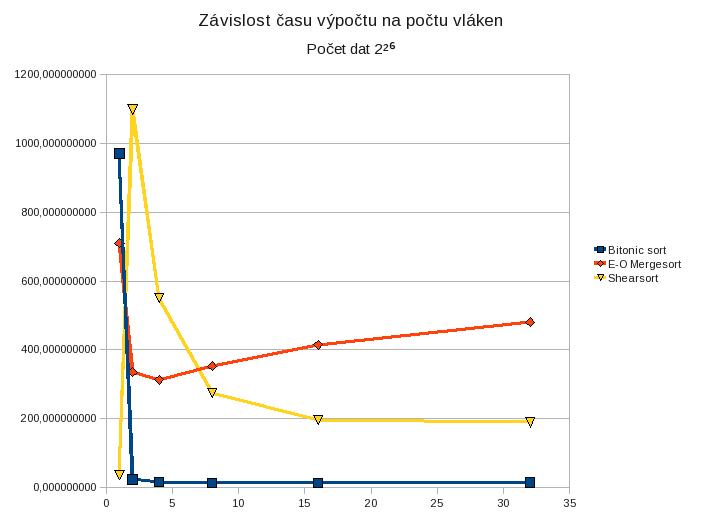
\includegraphics[width=14cm]{mereni.jpg}
\caption{Graf závislosti času na počtu vláken.}
\label{fig:testAinfib}
\end{center}
\end{figure}

\subsubsection{Zrychlení}
\begin{figure}[H]
\begin{center}
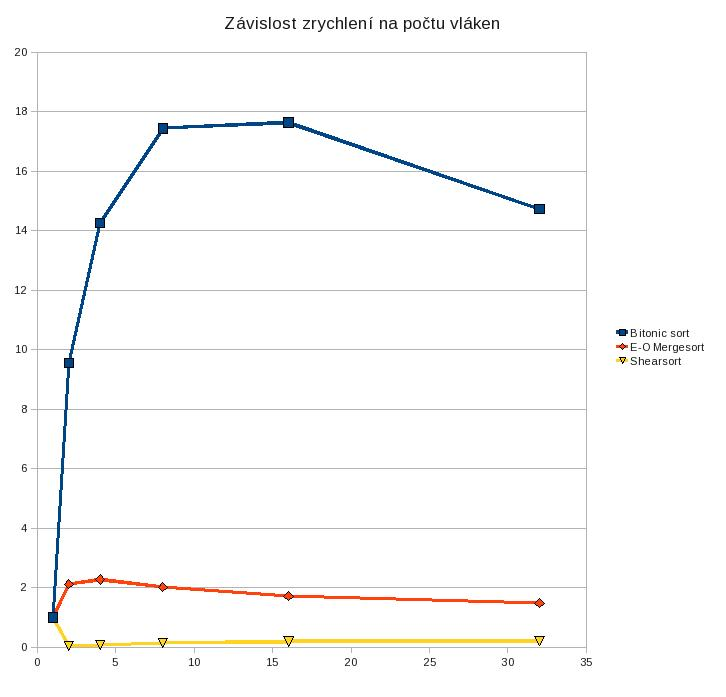
\includegraphics[width=14cm]{mereni2.jpg}
\caption{Zrychlení výpočtu v závisosti na počtu vláken.}
\label{fig:testAinfib}
\end{center}
\end{figure}



\begin{comment}
\begin{figure}[H]
\begin{center}
%\includegraphics[width=8cm]{grafy-zprava/testBinfib.png}
\caption{Test B}
\label{fig:testBinfib}
\end{center}
\end{figure}

\begin{figure}[H]
\begin{center}
%\includegraphics[width=8cm]{grafy-zprava/testCinfib.png}
\caption{Test C}
\label{fig:testCinfib}
\end{center}
\end{figure}

\subsection{Propojovací síť Ethernet}
Grafy závislosti času na počtu procesorů při použití propojovací sítě Ethernet.
\begin{figure}[H]
\begin{center}
%\includegraphics[width=8cm]{grafy-zprava/testAeth.png}
\caption{Test A}
\label{fig:testAether}
\end{center}
\end{figure}

\begin{figure}[H]
\begin{center}
%\includegraphics[width=8cm]{grafy-zprava/testBeth.png}
\caption{Test B}
\label{fig:testBether}
\end{center}
\end{figure}

\begin{figure}[H]
\begin{center}
%\includegraphics[width=8cm]{grafy-zprava/testCeth.png}
\caption{Test C}
\label{fig:testCether}
\end{center}
\end{figure}

\section{Grafy zrychlení}
Grafy zobrazující závislost zrychlení výpočtu na počtu procesorů.
\begin{figure}[H]
\begin{center}
%\includegraphics[width=8cm]{grafy-zprava/zrychleniinf.png}
\label{fig:zrychleniinf}
\caption{InfiniBand}
\end{center}
\end{figure}

\begin{figure}[H]
\begin{center}
%\includegraphics[width=8cm]{grafy-zprava/zrychlenieth.png}
\label{fig:zrychlenieth}
\caption{Ethernet}
\end{center}
\end{figure}
\end{comment}

\end{document}
